\definecolor{seabornblue}{rgb}{0.2980392156862745, 0.4470588235294118, 0.6901960784313725}
\definecolor{seaborngreen}{rgb}{0.3333333333333333, 0.6588235294117647, 0.40784313725490196}
\definecolor{seabornred}{rgb}{0.7686274509803922, 0.3058823529411765, 0.3215686274509804}

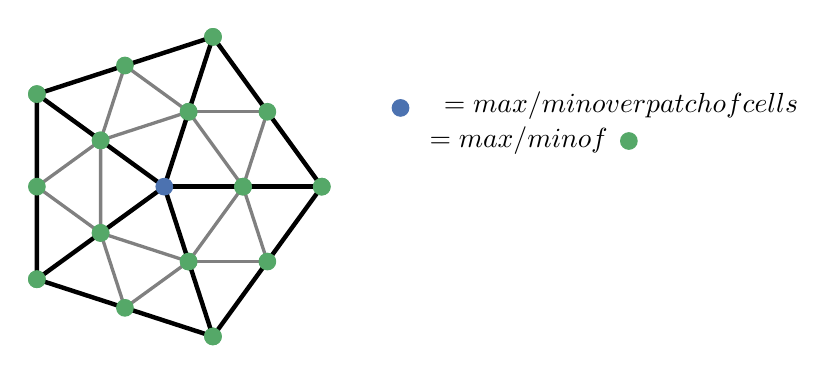
\begin{tikzpicture}[scale=2.0]
  \foreach \k in {0, 1, 2, 3, 4} {
    %\filldraw[seabornblue, fill=seabornblue] ({cos(deg(2*\k*pi/5))}, {sin(deg(2*\k*pi/5))}) circle (1.5pt);
    \node (A) at ({0.5*cos(deg(2*\k*pi/5)) + 0.5*cos(deg(2*(\k+1)*pi/5))}, {0.5*sin(deg(2*\k*pi/5)) + 0.5*sin(deg(2*(\k+1)*pi/5))}) {};
    \node (B) at ({0.5*cos(deg(2*\k*pi/5))}, {0.5*sin(deg(2*\k*pi/5))}) {};
    \node (C) at ({0.5*cos(deg(2*(\k+1)*pi/5))}, {0.5*sin(deg(2*(\k+1)*pi/5))}) {};
    \node (D) at ({cos(deg(2*\k*pi/5))}, {sin(deg(2*\k*pi/5))}) {};
    \node (E) at ({cos(deg(2*(\k+1)*pi/5))}, {sin(deg(2*(\k+1)*pi/5))}) {};

    \draw [-,gray, very thick] (A.center) -- (B.center);
    \draw [-,gray, very thick] (B.center) -- (C.center);
    \draw [-,gray, very thick] (C.center) -- (A.center);

    \draw [black, ultra thick] (0, 0) -- (D.center);
    \draw [black, ultra thick] (D.center) -- (E.center);

    \filldraw[seaborngreen] (A) circle (1.5pt);
    \filldraw[seaborngreen] (B) circle (1.5pt);
    \filldraw[seaborngreen] (C) circle (1.5pt);
    \filldraw[seaborngreen] (D) circle (1.5pt);
    \filldraw[seaborngreen] (E) circle (1.5pt);

  }
  \filldraw[seabornblue] (0, 0) circle (1.5pt);
  \node (expl) at (1.5, 0.5) {};
  \filldraw[seabornblue] (expl) circle (1.5pt);
  \node at (2.9, 0.5125) {$= \text{max/min over patch of cells}$};  % I'm sure there's a better way to place this, but tikz mystifies me
  \node at (2.25, 0.2925) {$= \text{max/min of }$};  % I'm sure there's a better way to place this, but tikz mystifies me
  \filldraw[seaborngreen] (2.95, 0.29) circle (1.5pt);
\end{tikzpicture}
